\documentclass[10pt,openany]{report}
\usepackage[a4paper,margin=1in]{geometry}
\usepackage{lmodern}
\usepackage[T1]{fontenc}
\usepackage{textcomp}
\usepackage{amsmath,amssymb}
\usepackage{graphicx}
\usepackage{booktabs}
\usepackage{array}
\usepackage{longtable}
\usepackage{multicol}
\usepackage{float}
\usepackage{tikz}
\usepackage{xcolor}
\usepackage{setspace}
\usepackage{caption}
\usepackage{hyperref}
\usetikzlibrary{shapes.geometric,arrows.meta,positioning,fit,backgrounds,calc,decorations.pathreplacing}

\hypersetup{
  colorlinks=true,
  linkcolor=black,
  citecolor=black,
  urlcolor=blue!45!black,
  pdftitle={GlandersWatch: A Modular Platform for Glanders Risk Prediction, Retrieval-Augmented Explanation and Owner Alerting},
  pdfauthor={Pedapatruni Shanmuk Vardhan, Shaktimayee Mohanty, Yuvraj Singh},
  pdfsubject={B.Tech Project Report, International Institute of Information Technology, Bhubaneswar}
}

\graphicspath{{../figures/}}
\captionsetup{font=small,labelfont=bf,skip=6pt}
\setlength{\parskip}{0.35em}
\setlength{\parindent}{0pt}
\setlength{\emergencystretch}{1.5em}
% single spacing, as in the department template

% Section numbering follows the department template: sections are "1.", "2." within
% each chapter (counter resets per chapter) and subsections are "1.1", "1.2".
\renewcommand{\thesection}{\arabic{section}.}
\renewcommand{\thesubsection}{\arabic{section}.\arabic{subsection}}

% chapter-based numbering for floats and equations
\counterwithin{figure}{chapter}
\counterwithin{table}{chapter}
\renewcommand{\thefigure}{\thechapter.\arabic{figure}}
\renewcommand{\thetable}{\thechapter.\arabic{table}}

\input{diagstyles.tex}
\begin{document}
% The department template numbers continuously in arabic from the Certificate page,
% with the title page carrying no number, so Abstract falls on page 4.
\pagenumbering{arabic}
\setcounter{page}{0}

% ============================== TITLE PAGE ==============================
% Bold/regular pattern measured from the department template: the title is large but
% REGULAR weight; the four structural headings are bold; author names are bold with the
% roll numbers set regular in a second column. Names right-aligned, roll numbers
% left-aligned, as a tabular{rl}.
\begin{titlepage}
\thispagestyle{empty}
\begin{center}

{\huge GlandersWatch: A Modular Platform for\\[7pt]
Glanders Risk Prediction, Retrieval-Augmented\\[7pt]
Explanation and Owner Alerting\par}

\vspace{1.15cm}

{\Large\bfseries Project Report Submitted\par}
\vspace{0.30em}
{\normalsize in partial fulfillment of the requirements for the award of the\par}

\vspace{1.05cm}
{\Large\bfseries Bachelor of Technology\par}
\vspace{0.28em}
{\normalsize in\par}
\vspace{0.22em}
{\Large\bfseries Computer Science Engineering\par}

\vspace{0.95cm}
{\normalsize by\par}
\vspace{0.40em}
{\fontsize{10.9}{13.2}\selectfont
\begin{tabular}{@{}r@{\hspace{1.1em}}l@{}}
\bfseries Pedapatruni Shanmuk Vardhan & B123089 \\[1pt]
\bfseries Shaktimayee Mohanty & B123118 \\[1pt]
\bfseries Yuvraj Singh & B123153 \\
\end{tabular}\par}

\vspace{1.0cm}
{\normalsize Under the supervision of\par}
\vspace{0.32em}
{\fontsize{10.9}{13.2}\selectfont\bfseries Dr. Sangita Dhara\par}

\vspace{1.0cm}

\includegraphics[width=3.0cm]{iiit_logo.png}\par

\vfill

{\normalsize Department of Computer Science and Engineering\par}
\vspace{0.32em}
{\fontsize{10.9}{13.2}\selectfont\bfseries International Institute of Information Technology, Bhubaneswar\par}
\vspace{0.32em}
{\normalsize November 2026\par}

\vspace*{0.6cm}

\end{center}
\end{titlepage}

% ============================== CERTIFICATE ==============================
\newpage
\thispagestyle{empty}
\noindent\underline{\textbf{Certificate}}

\vspace{0.9cm}
\noindent
{\sloppy
This is to certify that the report entitled ``GlandersWatch: A Modular Platform for Glanders Risk
Prediction, Retrieval-Augmented Explanation and Owner Alerting'' submitted by \mbox{Pedapatruni Shanmuk Vardhan (B123089)}, \mbox{Shaktimayee Mohanty (B123118)} and \mbox{Yuvraj Singh (B123153)} to
International Institute of Information Technology, Bhubaneswar is a record of bonafide project work
under my supervision, and the report is submitted for the evaluation of the BTech
Degree Final-Semester Project.\par}

\vspace{1.5cm}
\noindent
Dr. Sangita Dhara\\[0.2em]
\underline{(Supervisor)}

% ============================== DECLARATION ==============================
\newpage
\thispagestyle{empty}
\noindent\underline{\textbf{Declaration}}

\vspace{0.9cm}
\noindent
We certify that

\begin{enumerate}
  \item The work contained in the report has been done by ourselves under the general supervision
        of our supervisor.
  \item The work has not been submitted to any other Institute for any degree or diploma.
  \item We have followed the guidelines provided by the Institute in writing the report.
  \item We have conformed to the norms and guidelines given in the Ethical Code of Conduct of the
        Institute.
  \item Whenever we have used materials (data, theoretical analysis, and text) from other sources,
        we have given due credit to them by citing them in the text of the report and giving their
        details in the references.
  \item Whenever we have quoted written materials from other sources, we have put them under
        quotation marks and given due credit to the sources by citing them and giving required
        details in the references.
\end{enumerate}

\vspace{2.5cm}
\noindent
\noindent
\begin{tabular}{@{}p{5.75cm}p{4.35cm}p{4.35cm}@{}}
\textbf{Pedapatruni Shanmuk Vardhan} & \textbf{Shaktimayee Mohanty} & \textbf{Yuvraj Singh} \\[0.12em]
B123089 & B123118 & B123153 \\
\end{tabular}

% ============================== ACKNOWLEDGMENTS ==============================
\newpage
\thispagestyle{empty}
\noindent\underline{\textbf{Acknowledgments}}

\vspace{0.9cm}
\noindent
We would like to express our sincere gratitude to our respected supervisor, Dr. Sangita Dhara, for the
invaluable guidance, support and encouragement given throughout this project. Her insights and
expertise were instrumental in shaping this work and helped us overcome numerous challenges. We are
also thankful to the faculty and staff of the Department of Computer Science and Engineering,
International Institute of Information Technology, Bhubaneswar, for providing the resources and a
conducive learning environment. Finally, we would like to thank our families and friends for their
unwavering support and understanding during the course of this project.

\vspace{2.5cm}
\noindent
\noindent
\begin{tabular}{@{}p{5.75cm}p{4.35cm}p{4.35cm}@{}}
\textbf{Pedapatruni Shanmuk Vardhan} & \textbf{Shaktimayee Mohanty} & \textbf{Yuvraj Singh} \\[0.12em]
B123089 & B123118 & B123153 \\
\end{tabular}

% ============================== ABSTRACT ==============================
\newpage
\pagestyle{plain}
\noindent\underline{\textbf{Abstract}}
\addcontentsline{toc}{chapter}{Abstract}

\vspace{0.7cm}
\noindent
Glanders is a bacterial zoonosis of equids caused by \textit{Burkholderia mallei}. It is
notifiable, frequently fatal, and remains endemic in parts of Africa, Asia and South America.
Indian surveillance between 2019 and 2023 identified 728 seropositive equids across 138 districts,
with strong geographic concentration. The published machine learning literature on this disease is
confined to laboratory identification of the organism by spectroscopic methods, and no
population-level geographic risk model has been reported.

\vspace{0.5em}
\noindent
This report presents GlandersWatch, a platform built from three independently deployable components:
a calibrated machine learning risk engine, a retrieval-augmented layer that explains each
prediction with citations to official guidance, and an alert service that delivers the result to
equine owners. The decomposition is the contribution as much as the model is. Each component
communicates through a versioned schema rather than shared internals, none hardcodes the disease,
and each degrades without failing the others.

\vspace{0.5em}
\noindent
The risk engine combines four public datasets not previously applied to glanders into a country-year
panel: a text-mined occurrence corpus from Europe PMC, FAOSTAT livestock stocks, World Bank
development indicators and NASA POWER reanalysis climatology. The panel contains 3,078 country-year
observations across 162 equine-holding countries from 2005 to 2023, with 172 positive labels and 44
engineered features. Six model families are trained under three validation schemes, and a
three-stage chained pipeline is evaluated in which animal population is forecast before occurrence
is predicted.

\vspace{0.5em}
\noindent
On a forward temporal holdout the strongest model reaches a precision-recall AUC of 0.554 against a
base rate of 0.056, roughly a ten-fold lift, with an expected calibration error of 0.016. Performance
falls to 0.304 under leave-country-out validation, which is the estimate to quote for an unseen
country. Chaining produces no measurable gain in discrimination. An ablation shows climate
covariates transfer poorly across countries, and the model performs least well in low-income
regions. The dominant limitation is that the label reflects documented activity rather than true
incidence, so the model largely learns where disease is reported. Reporting effort is the principal
confounder and the main target for future work. The explanation and alert components are specified
to the level of their interfaces, rule semantics and evaluation protocol, and are not reported as
measured results because they are not deployed.

\vspace{0.7em}
\noindent
\textbf{Keywords:} Glanders, \textit{Burkholderia mallei}, Risk Prediction, Gradient Boosting,
Probability Calibration, SHAP, Retrieval-Augmented Generation, Citation Grounding, Alert Fatigue,
Modular System Design, MLOps, Animal Health Surveillance.

% ============================== CONTENTS ==============================
\newpage
\pagestyle{plain}
\noindent\underline{\textbf{Contents}}
\vspace{0.55cm}

% \tableofcontents would insert its own chapter-style heading and a page break;
% \@starttoc typesets the entries alone, under the heading above.
\makeatletter
\@starttoc{toc}
\makeatother

% =====================================================================
\chapter{Introduction}
\label{ch:intro}
% =====================================================================

\section{Background}

Glanders is a contagious and often fatal disease of horses, donkeys and mules caused by
\textit{Burkholderia mallei}. The organism has no environmental reservoir, and asymptomatic
carriers remain infectious for long periods. Human infection is rare but carries a high case
fatality rate and follows occupational contact. The disease is notifiable to the World
Organisation for Animal Health and is classified as a potential bioterrorism agent.

The economic weight of the disease sits in low and middle income countries, where equids remain
essential to transport, construction, agriculture and brick manufacture. India recorded 5.44 lakh
equids in the 2019 Livestock Census, many held by households that depend on them for daily income.
The loss of a working animal is a direct loss of livelihood, which makes early warning useful even
where mass treatment is not feasible.

Surveillance data show the disease is neither rare nor geographically contained. A national
programme screening 158,798 equid sera from 391 districts between 2019 and 2023 found 728
seropositive animals in 138 districts, with roughly sixty per cent of positives in Uttar Pradesh.
Earlier surveillance covering 2006 to 2018 reported 1,145 positive equids among 128,404 sera
tested. These are persistent, spatially structured figures, not isolated outbreaks.

\section{Problem Definition}

A district veterinary officer faces a narrow question: is glanders likely to appear in this area
in the coming year? Answering it means combining the history of the disease nearby, the size of
the susceptible population, and the conditions that permit transmission.

Surveillance reports what has already happened. Forecasting systems exist for several livestock
diseases but not for glanders. The problem addressed here is to build a population-level risk
model for glanders from public data and to measure how well it works. It has four parts:

\begin{enumerate}
  \item \textbf{Data assembly.} No public source records glanders occurrence completely. Occurrence
        must be reconstructed from the literature and joined to population and environmental
        covariates at a common resolution.
  \item \textbf{Label construction.} The outcome is rare, so accuracy is useless and a negative
        observation needs an explicit meaning.
  \item \textbf{Model selection under distribution shift.} A model fitted on some countries must be
        evaluated on countries it has never seen, because that is the deployment condition.
  \item \textbf{Threshold economics.} A probability is not an alert. The operating point must be
        defensible against the number of warnings it produces.
\end{enumerate}

\section{Objectives}

There is one research objective and three engineering objectives.

\begin{enumerate}
  \item \textbf{Research.} Assemble a country-year panel for glanders from public sources not
        previously applied to the disease, compare six model families under three validation
        schemes, and report the achievable skill, including negative results.
  \item \textbf{Prediction as a service.} Package the trained model as a versioned, portable
        artefact behind a REST interface, so any consumer can call it without knowing how it works.
  \item \textbf{Cited explanation.} Build a retrieval-augmented layer that explains a prediction
        from official guidance, cites every claim, and refuses rather than guesses.
  \item \textbf{Owner alerts.} Convert a calibrated probability into a small number of messages,
        using threshold, suppression and deduplication rules so that a rare disease does not train
        its users to ignore warnings.
\end{enumerate}

All four share one requirement: each component must be independently testable, independently
replaceable, and free of any hardcoded reference to glanders, so the platform can be repointed at
another disease without altering the components.

\section{Scope and Limitations}

The study is scoped to country-year resolution. District-level modelling for India was envisaged
in the project proposal but is not attempted, because the required covariates could not be
assembled from public sources within the project period. The explanation and alert layers are
resolution-agnostic and apply unchanged once a district-level model exists. The model is a
population-level tool: it does not diagnose an individual animal and does not replace laboratory
confirmation.

Three limitations shape every result that follows. The label comes from published reports, so a
negative may mean no disease or no reporting. Occurrence is reconstructed by an automated extractor
that has not been validated against a hand-annotated set. And with 172 positive observations the
uncertainty on every headline metric is substantial, which is quantified rather than hidden.

% =====================================================================
\chapter{Literature Review and Gap Analysis}
\label{ch:lit}
% =====================================================================

\section{Epidemiology and Surveillance}

Glanders is treated as a neglected zoonosis with high case fatality and a real occupational risk to
handlers \cite{khan2013,kanani2026}. A recent systematic review and meta-analysis consolidates
seroprevalence estimates and identifies management practice and animal movement as the dominant
drivers \cite{purnama2026}; regional reviews document continued circulation in Brazil
\cite{mota2022}. The disease persists where equid populations are large, animals move often and
surveillance is weak. The first two are measurable from public data, while the third decides whether
the disease is visible at all and is therefore a confounder rather than a covariate.

Indian surveillance is the strongest evidence base. Malik et al. described outbreaks reported
between 2006 and 2011 \cite{malik2012}, Singha et al. reported serological surveillance for 2015 to
2018 \cite{singha2020}, and the national programme covering 2019 to 2023 produced a prevalence
estimate with a risk analysis \cite{singha2026}. These establish where glanders occurs and which
animal-level factors the risk analysis identified. None builds a predictive model, and none uses
population or reanalysis covariates as predictors.

\section{Existing Forecasting Systems in India}

The closest operational system is NADRES v2, the National Animal Disease Referral Expert System run
by ICAR-NIVEDI \cite{nadres}. It combines outbreak records from AICRP centres with meteorological and
remote-sensing covariates and issues district-level forewarnings about two months ahead, using a
model family that overlaps with the one used here.

This project differs in four complementary ways. It is glanders-specific, where a national system
must spread effort across many diseases. It uses only public data, so anyone can reproduce and audit
it. It attaches a cited explanation to each prediction, which matters when the reader is an owner
rather than a trained analyst. And it delivers to the owner directly, with rules that suppress
routine noise. NADRES has institutional access this project lacks; this project has a level of local
explainability that a multi-disease platform does not attempt. The comparison also confirms that the
architecture chosen here is conventional for this problem class, and that the open question is not
whether to forecast but how to make a forecast understandable where it is used.

\section{Spatial Risk and Machine Learning}

Spatial work on glanders is descriptive. Fonseca-Rodr\'iguez et al. applied spatiotemporal cluster
detection to Brazilian data \cite{fonseca2019}, and species distribution models have been compared as
tools for livestock disease \cite{hollings2017}. Cluster detection identifies where cases have already
concentrated; it does not forecast which cells will be positive next period, which is the question an
early warning system must answer.

Predictive modelling is established for avian influenza. Kane et al. compared ARIMA and random forest
models for H5N1 outbreaks \cite{kane2014}, Walsh et al. used machine learning to target active
surveillance \cite{walsh2019}, and Yoo et al. and Alshatti et al. built farm-level risk models in Korea
and Kuwait \cite{yoo2022,alshatti2026}. That literature supplies the methodological template used
here: assemble occurrence, population and environmental covariates at a common unit, fit tree-based
ensembles, and evaluate on held-out periods. The template has been applied to influenza, not to
glanders.

The only machine learning work specific to \textit{B. mallei} is spectroscopic identification. Moawad
et al. built a Raman assay in which learned models classify spectra \cite{moawad2019}, and St\"ockel et
al. reported spectroscopic detection of \textit{B. mallei} and \textit{B. pseudomallei}
\cite{stoeckel2015}. Both are laboratory diagnostic problems; neither addresses geographic or temporal
distribution, and neither produces a population risk estimate. Using published literature as
structured occurrence data has precedent in epidemic intelligence \cite{collier2012,lejeune2015}, but
here event extraction is the primary source of the label rather than a supplementary signal, because
official outbreak records are incomplete for many countries. The label therefore inherits the
reporting biases of the literature, which is analysed rather than assumed away.

\section{Prior Art Audit}

To test the novelty claim rather than assert it, a reproducible set of queries was run against Europe
PMC. Each row of Table~\ref{tab:novelty} is a query count; the query strings and retrieved titles are
retained with the project code.

\begin{table}[htbp]
\centering
\caption{Europe PMC hit counts for combinations of glanders with each data source and method used
in this study.}
\label{tab:novelty}
\small
\begin{tabular}{@{}lc@{}}
\toprule
\textbf{Query} & \textbf{Hits} \\
\midrule
glanders (baseline corpus) & 6674 \\
glanders + machine learning & 75 \\
glanders + tree ensembles & 40 \\
glanders + forecasting & 139 \\
glanders + FAOSTAT & 7 \\
glanders + NASA POWER & 0 \\
glanders + World Bank indicators & 22 \\
glanders + equine population denominator & 54 \\
glanders + Europe PMC text mining & 378 \\
glanders + chained/stacked models & 36 \\
glanders + random forest (risk context) & 8 \\
glanders + niche / distribution model & 62 \\
glanders + remote sensing / reanalysis & 10 \\
glanders + spatio-temporal clustering & 463 \\
glanders + gradient boosting & 4 \\
\bottomrule
\end{tabular}
\end{table}

The decisive cells pair glanders with NASA POWER, which returns zero records, and with gradient
boosting, which returns four, none of them a glanders risk model. The nearest prior work is
descriptive cluster detection in Brazil and a risk-factor analysis of the Indian serosurvey.

\section{Research Gap}

The literature divides into three disjoint groups. Epidemiological studies describe where glanders
occurs; machine learning studies of \textit{B. mallei} classify laboratory spectra; veterinary risk
models exist but are built for influenza. No study joins an occurrence corpus, a livestock census,
development indicators and reanalysis climatology into a single panel for glanders, and none
evaluates a calibrated predictive model on that panel.

A second gap appears once the question moves from analysis to use. A probability on a dashboard does
not reach the person who owns the animals, and a risk score without a stated basis is not something a
field officer will act on. Both bodies of literature stop short of the delivery problem: how a
forecast becomes a cited explanation, and how that becomes a message an owner receives and trusts.

The contribution has two parts: a calibrated population-level risk model for glanders, built on data
sources not previously applied to the disease and evaluated under forward temporal and country-holdout
splits; and a decomposition of the delivery problem into three components with fixed contracts, so
prediction, explanation and alert can be built, tested and replaced independently.

% =====================================================================
\chapter{System Architecture}
\label{ch:arch}
% =====================================================================

\section{What the Platform Has to Do}

The platform answers one question and produces three outputs: whether glanders is likely to be
documented in an area next period, expressed as a number on a map, an explanation in words, and a
message to an owner. Each is read by a different person, at a different time, through a different
device, and each can fail without the others failing.

That asymmetry is why the system is three components rather than one application. One service serving
all three would tie alert delivery to the latency of an LLM call and make the risk model impossible to
test on its own.


\begin{figure}[htbp]
\centering
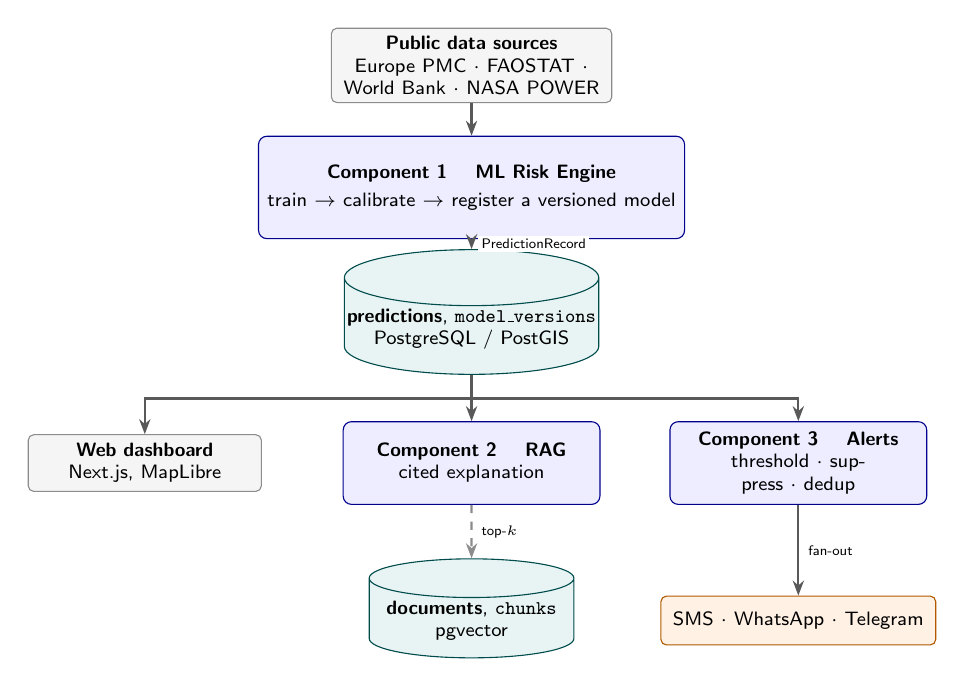
\begin{tikzpicture}[
  comp/.style={rectangle,rounded corners=3pt,draw=blue!55!black,fill=blue!7,
               align=center,minimum height=1.05cm,text width=3.35cm,
               font=\scriptsize\sffamily,inner sep=3pt},
  ext/.style={rectangle,rounded corners=2pt,draw=black!45,fill=black!4,
              align=center,minimum height=0.72cm,text width=3.35cm,
              font=\scriptsize\sffamily,inner sep=3pt},
  store/.style={cylinder,draw=teal!60!black,fill=teal!9,shape border rotate=90,
                aspect=0.22,minimum width=3.1cm,minimum height=1.15cm,
                font=\scriptsize\sffamily,align=center,inner sep=1pt},
  chan/.style={rectangle,rounded corners=2pt,draw=orange!70!black,fill=orange!10,
               align=center,minimum height=0.62cm,text width=3.35cm,
               font=\scriptsize\sffamily,inner sep=2pt},
  fl/.style={-{Stealth[length=1.9mm]},thick,draw=black!65},
  dfl/.style={-{Stealth[length=1.9mm]},thick,dashed,draw=black!45},
  clbl/.style={font=\tiny\sffamily,fill=white,inner sep=1.2pt,align=center},
]

  % ---- sources -----------------------------------------------------------
  \node[ext] (src) at (0,0)
    {\textbf{Public data sources}\\ Europe PMC $\cdot$ FAOSTAT $\cdot$ World Bank $\cdot$ NASA POWER};

  % ---- component 1 -------------------------------------------------------
  \node[comp,minimum height=1.30cm,text width=5.2cm] (c1) at (0,-1.55)
    {\textbf{Component 1 \quad ML Risk Engine}\\[2pt]
     train $\rightarrow$ calibrate $\rightarrow$ register a versioned model};

  % ---- prediction store --------------------------------------------------
  \node[store] (db) at (0,-3.35)
    {\textbf{predictions}, \texttt{model\_versions}\\
     PostgreSQL / PostGIS};

  % ---- the three consumers ----------------------------------------------
  \node[ext,text width=2.75cm] (dash) at (-4.15,-5.05)
    {\textbf{Web dashboard}\\ Next.js, MapLibre};

  \node[comp,text width=3.05cm] (c2) at (0,-5.05)
    {\textbf{Component 2 \quad RAG}\\ cited explanation};

  \node[comp,text width=3.05cm] (c3) at (4.15,-5.05)
    {\textbf{Component 3 \quad Alerts}\\ threshold $\cdot$ suppress $\cdot$ dedup};

  % ---- leaf stores -------------------------------------------------------
  \node[store,minimum width=2.6cm] (kb) at (0,-7.05)
    {\textbf{documents}, \texttt{chunks}\\ pgvector};
  \node[chan] (ch) at (4.15,-7.05)
    {SMS $\cdot$ WhatsApp $\cdot$ Telegram};

  % ---- edges -------------------------------------------------------------
  \draw[fl] (src) -- (c1);
  \draw[fl] (c1) -- node[clbl,right=2pt]{PredictionRecord} (db);

  \draw[fl] (db.south) -- ++(0,-0.30) -| ([xshift=-0.0cm]dash.north);
  \draw[fl] (db) -- (c2);
  \draw[fl] (db.south) -- ++(0,-0.30) -| (c3.north);

  \draw[dfl] (c2) -- node[clbl,right=2pt]{top-$k$} (kb.north);
  \draw[fl] (c3) -- node[clbl,right=2pt]{fan-out} (ch.north);

\end{tikzpicture}
\caption{The platform decomposed into three components. The ML risk engine
writes one \texttt{PredictionRecord} per area and period; the dashboard, the RAG
layer and the alert service consume it independently. No component reads another
component's tables, so any one of them can be replaced without touching the other
two.}
\label{fig:arch}
\end{figure}


\section{Design Principles}

Five rules govern the decomposition. Every later design decision follows from them, and they are
the part of the project that transfers to other diseases.

\textbf{One responsibility per component.} The risk engine turns features into a calibrated
probability, the RAG layer turns a prediction into a cited explanation, and the alert service turns
a prediction into a delivered message. None computes what another could compute instead.

\textbf{Contracts before implementations.} Components exchange versioned schemas, never shared
tables or in-process calls, so each side can be built and tested against a fixture. This is what let
the RAG layer be developed while the alert service was still being written.

\textbf{The core is disease-agnostic.} A disease is a configuration record: which label extractor,
knowledge-base collection, templates and thresholds to use. A second disease is a configuration
change plus a retrain, not a code fork.

\textbf{Fail soft, never fail silent.} A degraded component returns a degraded answer. If the RAG
layer is unavailable the alert still goes out, with the level and standing action text but no
explanation. If retrieval finds nothing above the relevance floor, the layer returns a refusal plus
the model's own SHAP factors. Neither case produces a wrong statement, and neither produces silence.

\textbf{Every output is traceable.} Each prediction carries its model version, each explanation the
document identifiers it was grounded in, each alert the prediction that triggered it and the rule
outcomes that allowed it, so a decision can be reconstructed after the fact.

\section{The Three Components}

\begin{table}[htbp]
\centering
\caption{Component responsibilities, interfaces and failure behaviour.}
\label{tab:components}
\small
\begin{tabular}{@{}>{\raggedright\arraybackslash}p{2.3cm}>{\raggedright\arraybackslash}p{3.5cm}>{\raggedright\arraybackslash}p{3.4cm}>{\raggedright\arraybackslash}p{4.2cm}@{}}
\toprule
\textbf{Component} & \textbf{Responsibility} & \textbf{Interface} & \textbf{On failure} \\
\midrule
ML risk engine & Features to calibrated probability, with attribution & \texttt{POST /v1/predict}, \texttt{GET /v1/risk-map} & \texttt{503} with the champion version id; the last good prediction stays in the table, marked stale. \\
RAG layer & Prediction plus question to a cited explanation & \texttt{POST /v1/explain}, \texttt{POST /v1/chat} & Alert text is sent without the explanation; chat returns a refusal rather than an ungrounded answer. \\
Alert service & Prediction to a delivered, deduplicated message & \texttt{POST /v1/alerts/evaluate}; consumes \texttt{predictions\_ready} & Alerts queue in Redis and drain on recovery; map and explanations are unaffected. \\
\bottomrule
\end{tabular}
\end{table}

\section{Component Contracts}

A contract is a JSON schema plus the guarantees that accompany it. A narrow contract is what makes
a component replaceable, so all three are deliberately small.

The risk engine emits a \texttt{PredictionRecord} with the area, period, calibrated probability,
discrete risk level, model identifier, a data-freshness block and the top SHAP factors. Three
guarantees accompany it: the probability is calibrated on held-out data and may be read as a
frequency; the risk level is derived from that probability by the threshold configuration, so the
two cannot contradict each other; and the top factors come from the model itself, so they remain
available when the RAG layer does not.

The RAG layer takes an \texttt{ExplainRequest}, wrapping a prediction with a question and a
language, and returns an \texttt{ExplainResponse} with an answer, resolved citations, a
\texttt{grounded} flag and a refusal reason. A refusal carries no answer text, so a caller cannot
render one as an explanation.

The alert service emits an \texttt{AlertEvent} with the alert identifier, area, period, current and
previous level, the prediction it derives from, each rule outcome and a recipient count. The
identifier is derived deterministically from its key (Chapter~\ref{ch:alerts}).

The components share a database but not tables: each table has one owning writer and the others
read it, and no component updates another's rows. Spatial columns use PostGIS and document
embeddings use pgvector, so spatial and vector queries run beside the relational joins rather than
in a second store that would need synchronising.

\section{Modularity and Reuse}

The decomposition justifies its overhead only if the parts are reusable. A second disease supplies a
new gazetteer, guidance collection and thresholds, while the modelling code, which never refers to
glanders by name, does not change. A second LLM provider is a configuration value, because the RAG
layer calls a single-method interface. A second channel is an adapter plus a template, and the rules
engine never learns which channel carries the message. The trained pipeline is a scikit-learn
compatible object \cite{pedregosa2011} exported with a manifest, so any Python process can load it
without the API. A replacement model needs no downstream change, since the record carries
\texttt{model\_id} and the registry keeps previous versions.

\section{Deployment and Status}

One Docker Compose file describes the API, worker, PostgreSQL with PostGIS and pgvector, Redis and the
frontend, so local demonstration and server deployment share a structure. A Celery beat job runs the
feature job, then the prediction job, then publishes \texttt{predictions\_ready}, from which
explanations and alerts are computed; a failed explanation never blocks a prediction, and a failed
prediction never sends an alert about stale data.

The report distinguishes throughout between what has been built and what has been specified. The risk
engine is built and evaluated, and every number in Chapter~\ref{ch:results} is reproducible from the
committed scripts. Model serving, the RAG layer and the alert service are specified with fixed
contracts and stated protocols but are not deployed, so no measured performance is reported for them.

% =====================================================================
\chapter{Methodology}
\label{ch:method}
% =====================================================================

\section{Data Sources}

Four public sources are used: a literature index, a livestock census, a development indicator set and
a reanalysis climate archive \cite{europepmc,faostat,wdi,power}. None had previously been applied to
glanders risk modelling.

Europe PMC supplies the animal history: 6,674 records yielding 263 occurrence
events. FAOSTAT supplies animal population, 68,449 records covering seven stock series from 1961 to
2023. The World Bank supplies socio-economic context, ten development indicators and country
centroids for 217 countries from 2000 to 2024. NASA POWER supplies environment, six measures of
temperature, precipitation, humidity and wind at 211 centroids from 2005 to 2024.

Extracted events rise in volume after 2015, which reflects growth in open access veterinary
publishing as much as any change in incidence. This is one reason the label is treated as
documented activity throughout.

\section{Panel Construction}

All four sources are keyed on ISO 3166 alpha-3 code and calendar year, so they join once names are
reconciled. FAOSTAT is streamed from its 32\,MB compressed archive and filtered to the seven stock
series rather than loaded whole. Names are matched through \texttt{pycountry} with overrides for forms
such as ``T\"urkiye'' and ``C\^ote d'Ivoire'', and World Bank regional and global aggregates are
excluded by requiring a three-character ISO code, so rows such as ``World'' never enter the panel as
though they were countries.

The grid holds 6,700 country-year rows across 268 countries for 2000 to 2024.
Three restrictions produce the modelling matrix: only equine-holding countries, defined as a maximum
equid stock of at least one thousand; only 2005 to 2023; and only rows with an observable next-year
label. The result has 3,078 rows, 44 features and 172 positives.

Events are de-duplicated on country, year and source record identifier, so one paper reporting
several cases cannot contribute multiple counts. Missing values are median-imputed inside the training
pipeline, with a missing-indicator feature per affected column, so the test period cannot influence
imputed values. Missingness is low: 0.00\% for FAOSTAT, 1.68\% for the World Bank, 2.19\% for
climate, and 0.99\% overall, with no column above 5.8\%.

\section{Label Definition}

The target is binary: whether a glanders occurrence was documented in country $i$ during year $t+1$.
Occurrence is extracted from Europe PMC by matching, within one sentence, a country name from a
curated gazetteer and a term from an occurrence lexicon (\emph{outbreak}, \emph{case},
\emph{detected}, \emph{seropositive}, \emph{surveillance}). An event is recorded for the year in the
sentence, or the publication year where none is stated. Because the label depends on publication it
is termed \emph{documented activity}: a negative may mean no disease or no report, so the model
predicts surveillance-observable activity rather than biological presence.

\section{Feature Engineering}

Four groups are built from information available at year $t$ or earlier. Seven disease-history
features cover prior-year occurrence, a five-year total, years since the last event, and world and
regional activity shares. Fourteen population features cover log equid and livestock stocks, equid
share, density, growth and species counts. Ten climate features cover temperature, precipitation,
humidity and wind, each with an anomaly against the country's own expanding mean, separating unusual
conditions from latitude. Eleven socio-geographic features cover income, agriculture, GDP, rural
share, connectivity and population, and largely proxy surveillance capacity.

Three derived features need definition. Equid share is horses, asses and mules divided by total farm
animals. Livestock units apply weights of 0.8 for cattle and camels and 0.1 for small ruminants, so
one number expresses grazing pressure across species. Years since the last event uses 99 to denote no
event in the window.

Selection ran in two stages. Columns with mutual information below 0.002 and absolute Spearman
correlation below 0.02 were removed, then one member of each pair correlated at or above 0.90, plus a
column that was exactly the sum of three others, which a tree can construct itself. No projection was
applied: with 44 features and 3,078 rows the binding constraint is signal rather than
dimensionality, and Section~\ref{sec:ablation} shows reduced sets transfer better.

\section{Models}

Six families are compared. Logistic regression is the additive baseline with balanced class weights.
A single shallow decision tree is included because a non-specialist can read it. Random forest and
extra trees are bagged ensembles \cite{breiman2001}, differing in split randomisation; XGBoost and
LightGBM are boosted ensembles \cite{chen2016,ke2017}. Tuning used grouped cross-validation on
country. Neural networks were excluded: with 172 positives and 44 features a network
has more parameters than examples and would memorise the training period.

\section{Evaluation Design}

Three schemes answer different questions. A temporal holdout trains on 2005 to 2017 and tests on 2018
to 2023, with the test period never observed during fitting, which answers whether the model can be
used in following years. Leave-country-out uses five folds grouped by country, so every prediction is
for an unseen country; it answers whether the model transfers and it governs selection, being the
harsher test and the closer approximation of deployment. Repeated stratified cross-validation, five
folds three times, is a stability check.

Precision-recall AUC is the primary metric: at 5.59\% prevalence ROC-AUC is dominated by the
true-negative mass and overstates performance \cite{saito2015,davis2006}, so it is reported only for
comparability. Brier score and expected calibration error are reported because an uncalibrated
probability cannot support a threshold-based alert \cite{niculescu2005,huang2020}. Precision, recall,
specificity, F1 and the Matthews correlation use a threshold tuned on training data only, with
bootstrap percentile intervals over one thousand resamples. Grouped rather than random splitting is
essential, since a random row split would let the model memorise country identity \cite{roberts2017}.

\section{Leakage Controls}

Six controls apply: features use year $t$ or earlier and only the target uses $t+1$; the split is
chronological; hyperparameters are tuned inside training folds; calibration is fitted on training
folds only; the alert threshold is fixed on training; and imputation values and missing indicators
are generated inside the pipeline.

% =====================================================================
\chapter{MLOps and Model Serving}
\label{ch:mlops}
% =====================================================================

\section{From a Notebook to a Service}

A trained model is not a component until it can be called, versioned, monitored and replaced. Three
things must be true first. The model must be a portable artefact, so the object scored in evaluation
is the object served, with nothing re-fitted in between. Every prediction must name the version that
produced it. And the service must degrade predictably, so a bad release or a missing feature does not
produce confident nonsense. The project is a sequence of numbered scripts, each producing artefacts
consumed by the next, with every intermediate output cached so any stage can be re-run alone. That is
also what makes the pipeline inspectable: a reader can run one stage and check it before trusting the
next.

\section{The Model Bundle}

The unit of deployment is a directory, not a pickled object, because a pickle alone cannot say what
its inputs mean.

\begin{verbatim}
gw-xgb-2026.11.1/
  model.joblib        # fitted pipeline, predict_proba
  manifest.json       # feature order, dtypes, calibration, metrics
  thresholds.json     # level boundaries and hysteresis margin
  SHA256SUMS
\end{verbatim}

The manifest is what makes the bundle reusable. It records the ordered feature list with dtypes, so
serving rejects a request with the wrong columns before any inference happens. It records the
calibration method and achieved error, so a consumer knows whether to read the output as a probability
or only as a rank. It records the evaluation metrics, so the number in the report and the number in
the registry are the same. Because the bundle is a directory with a manifest, the API, a batch job and
a notebook load it with identical behaviour.

Every training run also writes a record with the git commit, data version, feature list and hash,
hyperparameters and the full metric set for all three schemes. Promotion is decided on
leave-country-out precision-recall AUC rather than on the more flattering temporal holdout. A
candidate becomes champion only if it beats the incumbent by more than the bootstrap interval width,
its expected calibration error is below the deployment ceiling of 0.05, its feature schema matches
what serving can supply when checked by name and order, and it has scored a shadow period without a
prediction outside the plausible range. The previous champion is retained, so promotion is reversible,
and a bundle failing its checksum or schema check is replaced by the previous champion rather than
served.

\section{Serving Design}

The interface is deliberately coarse: a caller asks for a prediction for an area and period and
receives the full record, rather than assembling one from several calls.

\begin{table}[htbp]
\centering
\caption{HTTP interface of the risk engine.}
\label{tab:api}
\small
\begin{tabular}{@{}>{\raggedright\arraybackslash}p{3.4cm}>{\raggedright\arraybackslash}p{1.4cm}>{\raggedright\arraybackslash}p{9.2cm}@{}}
\toprule
\textbf{Endpoint} & \textbf{Method} & \textbf{Purpose and contract} \\
\midrule
\texttt{/v1/predict} & POST & Score one area and period from a supplied or stored feature vector. Returns one \texttt{PredictionRecord}. \\
\texttt{/v1/predict/batch} & POST & Score up to 500 area-period pairs, with per-item errors rather than failing the request. \\
\texttt{/v1/risk-map} & GET & GeoJSON of the latest predictions for a period, filtered by risk level. Serves the dashboard directly. \\
\texttt{/v1/models} & GET & Registry listing: model id, promotion date, metrics, feature-schema hash. \\
\texttt{/v1/models/\{id\}} & GET & The manifest of one version, for inspection by a consumer. \\
\texttt{/v1/health} & GET & Liveness and readiness, where readiness checks that a champion bundle is loaded and its schema resolves. \\
\bottomrule
\end{tabular}
\end{table}

Every response carries the \texttt{model\_id} that produced it and a \texttt{data\_freshness} block.
The alert service reads that block before sending anything, so a prediction computed on stale
upstream data cannot produce a message.


The order of operations is a reliability choice. Validation runs first, so a malformed request costs a
schema check rather than a model load. The cache is consulted before
inference because risk maps are read far more often than recomputed. Inference is deterministic for a
fixed bundle, so a cache key of model id, area and period is safe, and the model id is part of the key
rather than a version counter so promotion invalidates the cache. Responses are written back to the
predictions table as well as cached, so the map does not depend on a warm cache.

The endpoint is specified against a budget rather than measured, since the service is not deployed:
40\,ms on a cache miss and 4\,ms on a hit, of which feature retrieval takes 25\,ms and inference 8\,ms.
The explanation endpoint has a separate budget of two seconds because it includes generation, which is
why the alert service never calls it inline. A message must not wait on an LLM.

\section{Monitoring and Retraining}

Three classes of signal are monitored. Service health covers request rate, error rate and latency
percentiles per endpoint on a Prometheus endpoint charted in Grafana, which catches the service being
down, the least interesting failure. Data drift compares each feature's current distribution with the
training distribution using a population stability index and a Kolmogorov-Smirnov statistic, because a
tree asked to extrapolate outside its training range returns a confident answer with no basis.
Prediction drift and calibration decay track the mean predicted probability per period against the
observed event rate as labels arrive: a model that keeps saying 0.2 while the observed rate falls to
0.05 has lost calibration even with its ranking intact.

Retraining follows from the third signal. Recalibrate when the observed-to-predicted ratio leaves a
band for two consecutive periods, and retrain when a new year of labels is available and the champion's
leave-country-out score has degraded beyond the bootstrap interval.

The pipeline runs linting, unit tests and a smoke test on every push. Unit tests cover what can be
checked without data: schema validation, the level-threshold function including hysteresis at the
boundary, idempotency key derivation, and the citation parser. A further test loads the committed
bundle, scores a fixed fixture and asserts the output to four decimals, which catches the most common
silent failure here, where a dependency upgrade changes numerical behaviour and every downstream number
moves unnoticed.

The full computation runs in about 4.5 minutes on an Apple M4 processor with 10 cores and 16 GB of unified memory without a graphics accelerator.
Per-family fitting time at the country-year level ranges from 1.9 seconds for the decision tree
to 50.7 seconds for LightGBM. One module-level seed governs fitting, cross-validation, bootstrap
resampling and SHAP sampling, with software versions Python 3.12.13, scikit-learn 1.9.1, XGBoost 3.4.1, LightGBM 4.7.0, SHAP 0.54.1, NumPy 2.5.4, pandas 3.1.1, SciPy 1.18.1, and the bundle smoke test runs
single-threaded because tree ensembles are not bitwise reproducible across thread counts.

% =====================================================================
\chapter{The RAG Explanation Layer}
\label{ch:rag}
% =====================================================================

\section{The Problem This Layer Solves}

A calibrated probability of 0.24 is actionable for a veterinary officer and meaningless to an equine
owner. The owner needs to know what happened, what it means for their animals, and what to do next.
The officer needs to know which factors drove the number, because a forecast they cannot interrogate
is a forecast they will not act on.

Asking a large language model is the obvious answer and the obvious hazard. A model asked about
glanders answers from training data that may be outdated, may conflate glanders with melioidosis,
and may invent a treatment protocol. For a zoonosis under statutory control, an invented instruction
is worse than no instruction. Retrieval-augmented generation \cite{lewis2020} changes what the model
may use: it is not asked what it knows, but given a small set of passages from official guidance
plus the prediction's own numbers, and required to answer only from those. Each claim traces to a
passage, and the passage is shown to the reader.

The goal is therefore narrow and testable: an answer a veterinary officer would accept as consistent
with the National Action Plan, and a refusal rather than a guess when the corpus does not support
one.

Fine-tuning would produce fluent text with no citations and no way to tell guidance from the base
model's priors, and it would freeze the knowledge at training time, so a revised plan would require
retraining. Retrieval keeps knowledge in a corpus that a re-ingestion can update, makes every answer
auditable by construction, and allows a refusal path that fine-tuning does not. The cost is latency
and possible retrieval failure, both handled explicitly below.

\section{Knowledge Base}

The corpus is restricted to sources with authority, because the layer's value is that it cites them.
Each document carries an authority tier, used as a tie-breaker during retrieval.

\begin{table}[htbp]
\centering
\caption{Knowledge base, by authority tier.}
\label{tab:corpus}
\small
\begin{tabular}{@{}>{\raggedright\arraybackslash}p{5.0cm}>{\raggedright\arraybackslash}p{1.6cm}>{\raggedright\arraybackslash}p{7.0cm}@{}}
\toprule
\textbf{Source} & \textbf{Tier} & \textbf{Use} \\
\midrule
DAHD National Action Plan for Glanders, 2025 \cite{dahd2025} & 1 & Case definitions, surveillance obligations, movement control, quarantine, notification duties. \\
WOAH and WHO disease information sheets & 1 & Disease biology, transmission, zoonotic risk, official status. \\
ICAR and national laboratory guidance & 2 & Diagnostic sampling, laboratory referral. \\
Open-access research papers & 3 & Epidemiology, risk factors, regional situation. \\
\bottomrule
\end{tabular}
\end{table}

Tier 3 may inform an explanation but never overrides tier 1 on a control instruction. When passages
conflict the higher tier wins and the conflict is logged, because a silent contradiction between
sources is exactly the failure this layer exists to prevent.

\section{Ingestion, Embedding and Retrieval}

Ingestion runs offline as a job. A document is parsed, split at section boundaries, and each chunk
is stored with enough metadata to be cited and filtered.

Chunking is section-aware rather than fixed-width, because a fixed window cuts control instructions
in half and lets the model complete a truncated sentence. The splitter respects headings first, then
paragraphs, and falls back to a sliding window only for a section longer than the ceiling. Chunks
target 400 to 700 tokens with 15 per cent overlap inside a section, sections under 80 tokens merge
into the parent, and the retained metadata is document id, title, full section path, page, year and
authority tier. The section path is kept in full, for example
\texttt{NAP-2025 > 5.2 Movement control}, so a citation points to a subsection rather than to a
90-page document.

Chunks are embedded with a compact sentence-transformer \cite{reimers2019} producing 384-dimensional
vectors, cheap enough to embed on a laptop, with a multilingual variant for Hindi because an
English-only embedding degrades on Devanagari. Vectors live in pgvector beside the relational tables,
so re-ingestion and prediction share one transaction boundary. The index is HNSW with cosine distance
\cite{malkov2020}, acceptable because the reranker corrects recall at the head of the list and it keeps
query cost flat as the corpus grows.


\begin{figure}[htbp]
\centering
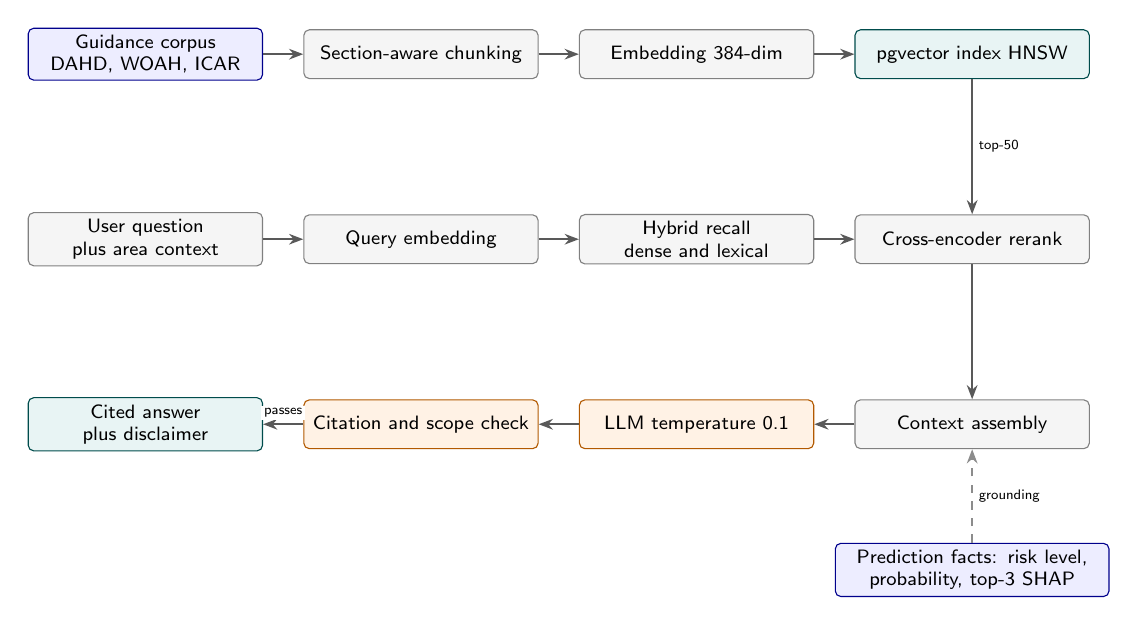
\begin{tikzpicture}[
  st/.style={rectangle,rounded corners=2pt,draw=black!50,fill=black!4,
             align=center,minimum height=0.62cm,text width=2.8cm,
             font=\scriptsize\sffamily,inner sep=2.5pt},
  doc/.style={rectangle,rounded corners=2pt,draw=blue!55!black,fill=blue!7,
              align=center,minimum height=0.62cm,text width=2.8cm,
              font=\scriptsize\sffamily,inner sep=2.5pt},
  gate/.style={rectangle,rounded corners=2pt,draw=orange!70!black,fill=orange!10,
               align=center,minimum height=0.62cm,text width=2.8cm,
               font=\scriptsize\sffamily,inner sep=2.5pt},
  emit/.style={rectangle,rounded corners=2pt,draw=teal!60!black,fill=teal!9,
               align=center,minimum height=0.62cm,text width=2.8cm,
               font=\scriptsize\sffamily,inner sep=2.5pt},
  fl/.style={-{Stealth[length=1.8mm]},thick,draw=black!65},
  dfl/.style={-{Stealth[length=1.8mm]},thick,dashed,draw=black!45},
  l/.style={font=\tiny\sffamily,fill=white,inner sep=1pt,align=center},
]
  % ---- offline ingestion, row 1 -----------------------------------------
  \node[doc] (corpus) at (0,0)      {Guidance corpus\ DAHD, WOAH, ICAR};
  \node[st]  (parse)  at (3.5,0)    {Section-aware\ chunking};
  \node[st]  (emb)    at (7.0,0)    {Embedding\ 384-dim};
  \node[emit] (idx)   at (10.5,0)   {pgvector index\ HNSW};

  % ---- online retrieval, row 2 ------------------------------------------
  \node[st] (q)   at (0,-2.35)   {User question\ plus area context};
  \node[st] (qe)  at (3.5,-2.35) {Query\ embedding};
  \node[st] (hyb) at (7.0,-2.35) {Hybrid recall\ dense and lexical};
  \node[st] (rr)  at (10.5,-2.35){Cross-encoder\ rerank};

  % ---- assembly and generation, row 3 (right to left) -------------------
  \node[st]   (ctx) at (10.5,-4.70) {Context\ assembly};
  \node[gate] (gen) at (7.0,-4.70)  {LLM\ temperature 0.1};
  \node[gate] (gd)  at (3.5,-4.70)  {Citation and\ scope check};
  \node[emit] (ans) at (0,-4.70)    {Cited answer\ plus disclaimer};

  \node[doc,text width=3.3cm] (facts) at (10.5,-6.55)
    {Prediction facts: risk level,\ probability, top-3 SHAP};

  \draw[fl] (corpus) -- (parse);
  \draw[fl] (parse) -- (emb);
  \draw[fl] (emb) -- (idx);

  \draw[fl] (q) -- (qe);
  \draw[fl] (qe) -- (hyb);
  \draw[fl] (hyb) -- (rr);

  \draw[fl] (idx) -- node[l,right=1pt]{top-50} (rr);
  \draw[fl] (rr) -- (ctx);
  \draw[fl] (ctx) -- (gen);
  \draw[fl] (gen) -- (gd);
  \draw[fl] (gd) -- node[l,above=1pt]{passes} (ans);

  \draw[dfl] (facts) -- node[l,right=1pt]{grounding} (ctx);
\end{tikzpicture}
\caption{The RAG layer. Ingestion (top row) is an offline job; retrieval, assembly and generation
(below) run per request. Predicted risk and SHAP factors are injected as structured facts, so the
answer explains this forecast rather than glanders in general. The citation check sits after
generation and can return a refusal instead of an unsupported answer.}
\label{fig:rag}
\end{figure}


Retrieval is hybrid, because dense and lexical search \cite{robertson2009} fail differently here. A
dense query for ``what should I do if I suspect glanders'' retrieves passages about suspicion, which
helps. A dense query for ``movement control'' may miss a passage using ``restriction of equid
movement'', where a lexical match succeeds; conversely a lexical query for a rare acronym retrieves
noise a dense query ignores. Both lists are retrieved and fused by reciprocal rank fusion
\cite{cormack2009}, which combines rankings without requiring comparable scores:

\[
\mathrm{RRF}(d) = \sum_{i \in \{\text{dense},\text{lexical}\}} \frac{1}{k + \mathrm{rank}_i(d)},
\qquad k = 60
\]

The fused top fifty are reranked by a cross-encoder scoring each passage against the question
jointly. A cross-encoder is far slower per pair than an embedding dot product, which is why it runs
on fifty candidates rather than on the corpus, and the top five become the context.

\begin{table}[htbp]
\centering
\caption{Retrieval parameters.}
\label{tab:retrieval}
\small
\begin{tabular}{@{}lll@{}}
\toprule
\textbf{Stage} & \textbf{Setting} & \textbf{Reason} \\
\midrule
Dense recall & top 30, cosine & Semantic paraphrase coverage \\
Lexical recall & top 30, BM25 & Exact terms, acronyms, section titles \\
Fusion & reciprocal rank, $k=60$ & Scale-free combination of two rankings \\
Rerank & cross-encoder, top 50 to 5 & Precision at the head of the list \\
Relevance floor & rerank score below 0.30 discarded & Prevents padding the context with weak passages \\
\bottomrule
\end{tabular}
\end{table}

The relevance floor drives the refusal path: if fewer than two passages clear it, the layer returns a
refusal with the SHAP factors, because a context built from marginal passages produces a confident
answer built on nothing.

\section{Context, Generation and Guardrails}

The prompt has three parts in fixed order: a system instruction, the retrieved passages with
identifiers, and the structured prediction facts. Those facts make the answer specific to this
forecast rather than to glanders in general, and they are injected as structured data so the model
cannot restate an association as a cause. The system instruction states four constraints: answer only
from the passages, cite every claim, never diagnose an individual animal, and state that the output is
a population-level forecast.

Generation uses temperature 0.1 and a bounded output length. Low temperature is chosen for
consistency rather than caution: two officers asking the same question about the same area should
receive the same instruction. The provider sits behind a single-method interface, so the same
retrieval, grounding and citation code runs against a local Ollama model or a hosted API, and
switching model cannot silently disable the guardrails.

The layer is designed to refuse, and four checks can terminate a response.

\begin{table}[htbp]
\centering
\caption{Guardrails and their failure behaviour.}
\label{tab:guardrails}
\small
\begin{tabular}{@{}>{\raggedright\arraybackslash}p{3.0cm}>{\raggedright\arraybackslash}p{5.2cm}>{\raggedright\arraybackslash}p{5.4cm}@{}}
\toprule
\textbf{Check} & \textbf{What it verifies} & \textbf{On failure} \\
\midrule
Retrieval floor & At least two passages above the relevance threshold & Refusal with the top SHAP factors, which need no retrieval \\
Citation resolution & Every cited identifier exists in the retrieved set & Answer rejected and regenerated once, then refusal \\
Diagnosis scope & No individual-animal diagnosis or treatment prescription & Response rewritten without the clinical claim, and the attempt logged \\
Out-of-scope & Question is about glanders control, not unrelated topics & Refusal stating what the layer covers \\
\bottomrule
\end{tabular}
\end{table}

The citation check is mechanical. The answer is parsed for identifiers and each is looked up in the
retrieved set; one that does not resolve means the model cited a document it was not given, which is a
hallucination whether or not the sentence is true. Asking a model to be accurate is not a control;
checking its output is.

\section{Evaluation}

Four quantities are measured, none of them whether the prose reads well. Retrieval quality is
recall@5 and mean reciprocal rank on a hand-built question set, which isolates retrieval from
generation, since no generation quality helps if the right passage is never retrieved. Faithfulness
is whether each claim is supported by the retrieved context, scored by a judge model and reviewed
by hand on a sample; this catches a model that cites a passage but says something it does not say.
Citation precision is the fraction of citations resolving to a passage that supports the sentence,
which is distinct from resolution, since resolution only checks existence. Refusal
behaviour is the refusal rate on out-of-scope questions and the false refusal rate in scope: a layer
that never refuses is unsafe and one that always refuses is useless, so both are reported.

Because the layer is specified rather than deployed, the validation that would precede deployment is
stated so the claim is falsifiable: recall@5 above 0.85, faithfulness above 0.90 on 100 manually
reviewed answers, citation precision above 0.95, zero individual-animal diagnoses on an adversarial
probe set, refusal on every out-of-scope question with a false refusal rate below 10 per cent, and
p95 latency under two seconds. These are targets, not results.

% =====================================================================
\chapter{The Alert Service}
\label{ch:alerts}
% =====================================================================

\section{Why the Alert Is the Hard Part}

The risk engine produces a probability and the RAG layer explains it, but neither reaches the person
who owns the animals, whose only interaction is a message on a phone competing with everything else
on it. The design problem is therefore not how to send a message but how to send few enough that the
ones which arrive are read. A system that warns about every area every month trains its users to
ignore it, then fails silently at the moment it was built for.

The service is event-driven: the prediction job publishes \texttt{predictions\_ready} and the evaluator
consumes it, so an alert cannot be sent for a period whose predictions were not recomputed. For each
subscribed area the evaluator reads the new prediction and the previous alert state, and those two
values are the entire input to the rules. It reads no features or model internals, so a model change
can affect alert behaviour only through the probability it produces.

\section{Rule 1: Threshold with Hysteresis}

The calibrated probability maps to three levels. The boundaries are configuration values derived
from the operating curve in Chapter~\ref{ch:results}, not defaults and not 0.5.

\begin{table}[htbp]
\centering
\caption{Level thresholds and their basis.}
\label{tab:thresholds}
\small
\begin{tabular}{@{}p{1.6cm}p{2.6cm}p{5.4cm}p{3.4cm}@{}}
\toprule
\textbf{Level} & \textbf{Band} & \textbf{Meaning for the recipient} & \textbf{Basis} \\
\midrule
LOW & below the medium boundary & No message. Routine monitoring. & Below the budget where precision collapses \\
MEDIUM & medium to high boundary & Prepare; check animals; note the veterinary contact & Operating point where recall exceeds 80 per cent \\
HIGH & above the high boundary & Act: restrict movement, isolate suspects, inform the authority & Top of the operating curve, precision above 0.5 \\
\bottomrule
\end{tabular}
\end{table}

Hysteresis addresses a specific defect. With a single boundary, an area whose probability oscillates
around the threshold produces an alert every period, because each crossing is a state change. Two
boundaries are therefore used: an area enters HIGH at the high threshold and leaves only when the
probability falls below that threshold minus a margin.

\[
\text{enter HIGH at } p \ge T_H, \qquad
\text{leave HIGH only at } p < T_H - \delta, \qquad \delta = 0.05
\]

The margin is configurable per disease. A larger margin gives a more stable state at the cost of
slower de-escalation, which suits a disease where a missed warning costs more than a late all-clear.

\section{Rule 2: Suppression}

Suppression decides whether a message is warranted at all, given that the level has changed. Six
conditions apply and any one can stop the message.

\begin{table}[htbp]
\centering
\caption{Suppression conditions.}
\label{tab:suppression}
\small
\begin{tabular}{@{}>{\raggedright\arraybackslash}p{3.0cm}>{\raggedright\arraybackslash}p{5.2cm}>{\raggedright\arraybackslash}p{5.4cm}@{}}
\toprule
\textbf{Condition} & \textbf{Rule} & \textbf{Rationale} \\
\midrule
State change & Send only on a transition, not while the level is held & A monthly reminder at the same level carries no new information \\
Cooldown & No repeat of the same level within a configurable window & Prevents oscillation at a boundary from producing repeated messages \\
Escalation bypass & An upward transition ignores the cooldown & A worsening must never be delayed by a timer \\
Per-user daily cap & At most one message per recipient per day & Protects against several areas escalating at once \\
Quiet hours & Nothing sent between 21:00 and 07:00 local; queued instead & A warning that wakes a household at night is resented, and is not actionable then \\
Stale-data guard & No send if \texttt{data\_freshness.passes} is false & An alert about a prediction computed on stale inputs is worse than no alert \\
\bottomrule
\end{tabular}
\end{table}

A manual mute per area lets an officer silence a zone under active surveillance without disabling the
service. De-escalation is separate: when a level falls, an optional short all-clear is sent, since a
recipient told to act needs to be told when to stop. Sending it is a configuration choice, because an
all-clear costs a message but prevents a restriction being maintained indefinitely.

\section{Rule 3: Deduplication}

The service must be safe to re-run: jobs are retried, deployments restart workers, and a model may be
re-scored for the same period, and none may produce a second message. Deduplication is enforced at
three levels, each with its own key and database constraint.

\begin{table}[htbp]
\centering
\caption{Deduplication levels.}
\label{tab:dedup}
\small
\begin{tabular}{@{}p{1.4cm}p{4.6cm}p{7.4cm}@{}}
\toprule
\textbf{Level} & \textbf{Key} & \textbf{What it prevents} \\
\midrule
Alert & \texttt{(area\_id, period, level)} & A re-run of the job creating a second alert for the same period \\
Recipient & \texttt{(alert\_id, subscription\_id)} & One subscriber receiving the same alert through two fan-out passes \\
Send & \texttt{(alert\_id, subscription\_id, attempt)} & A retry after a timeout delivering a message that had in fact succeeded \\
\bottomrule
\end{tabular}
\end{table}

The first two are unique database constraints, so protection does not depend on application logic
being correct. The alert identifier is derived deterministically from its key rather than at random,
so two concurrent workers computing the same alert arrive at the same identifier and one loses the
insert. The send-level check reads the delivery log before each attempt, handling the case where a
provider accepts a message, the response times out, and the retry would deliver it twice.

\section{Fan-Out, Channels and Delivery}

Once an alert record exists, one delivery job per subscription is queued through Redis. A channel
adapter receives a rendered message and a recipient and returns a delivery status, with adapters for
SMS, WhatsApp and Telegram, the last used for demonstration because it needs no commercial
onboarding. Retries use exponential backoff with jitter: a permanent failure such as an invalid number
is not retried, a transient one such as a provider timeout is, and the distinction is logged, because
a silent permanent failure leaves a subscriber who believes they are covered and is not. Templates are
separate from the rules engine, so adding a language adds a template set rather than touching the
rules.

The same alert through a richer channel carries the explanation paragraph from the RAG layer with its
citations. The rule that decides whether to send is identical; only the adapter and template differ,
which is what lets one alert serve a feature phone and a smartphone without duplicating the decision
logic.

\section{Evaluation of the Alert Layer}

The service is evaluated as a warning system, not as a messaging system. Alert precision is the
fraction of HIGH area-periods followed by a documented event, and it determines whether recipients
trust the message. Event coverage at budget is the operating curve already reported in
Chapter~\ref{ch:results}, and the thresholds are read from it. Noise per recipient is messages per
subscriber per year, which predicts whether the service will still be read in its second year.
Delivery reliability is the fraction of queued deliveries reaching a terminal success state within
the retry window, reported per channel. The first two come from historical predictions and labels;
the last two need a deployed service and are stated as the protocol that would measure them.

% =====================================================================
\chapter{Results and Discussion}
\label{ch:results}
% =====================================================================

\section{Dataset Characteristics}

The modelling matrix holds 3,078 country-year observations, of which 172 are positive: a
prevalence of 5.59\% and an imbalance of 16.9 to one. 56 of 162
countries record at least one positive, 30 of them in two or more years, and the top five
hold 35.5\% of all positives. The imbalance rules out accuracy as a metric and motivates
precision-recall analysis; the persistence justifies historical features; and the concentration is
the first indication that the label tracks reporting capacity, since those countries operate
reference laboratories.

\section{Model Comparison}

Table~\ref{tab:level1} reports discrimination under all three schemes.

\begin{table}[htbp]
\centering
\caption{Discrimination at the country-year level. Brackets give 95 per cent bootstrap intervals
on the temporal holdout.}
\label{tab:level1}
\small
\resizebox{\textwidth}{!}{%
\begin{tabular}{@{}lcccccccc@{}}
\toprule
\textbf{Model} & \textbf{PR-AUC} & \textbf{95\% CI} & \textbf{ROC-AUC} &
\textbf{PR-AUC} & \textbf{PR-AUC} & \textbf{Brier} & \textbf{Prec.} & \textbf{Rec.} \\
 & \textbf{(time)} & \textbf{on PR-AUC} & \textbf{(time)} & \textbf{(country)} &
\textbf{(rep.\ CV)} & & & \\
\midrule
Logistic regression & 0.454 & [0.34, 0.58] & 0.812 & 0.223 & 0.414 & 0.0547 & 0.25 / 0.57 \\
Decision tree & 0.389 & [0.29, 0.50] & 0.861 & 0.267 & 0.360 & 0.0602 & 0.49 / 0.53 \\
Random forest & 0.554 & [0.43, 0.66] & 0.870 & 0.304 & 0.476 & 0.0503 & 0.53 / 0.50 \\
Extra trees & 0.530 & [0.42, 0.64] & 0.854 & 0.363 & 0.476 & 0.0535 & 0.47 / 0.51 \\
XGBoost & 0.485 & [0.37, 0.60] & 0.844 & 0.281 & 0.423 & 0.0536 & 0.61 / 0.38 \\
LightGBM & 0.496 & [0.38, 0.61] & 0.841 & 0.339 & 0.397 & 0.0534 & 0.65 / 0.30 \\
\bottomrule
\end{tabular}}
\end{table}

Against a base rate of 5.59\%, the strongest temporal result of 0.554 is an approximately
10-fold lift. Every tree-based model beats the logistic baseline, and the single decision tree is
weakest, which indicates that the relationships are interactive rather than additive. The more
important pattern is the decline under leave-country-out validation: for Random Forest the score falls
from 0.554 to 0.304, and the decline exceeds the bootstrap interval width for every family. That
is the signature of learning country-specific structure, and the estimate to quote for deployment.

\begin{figure}[htbp]
\centering
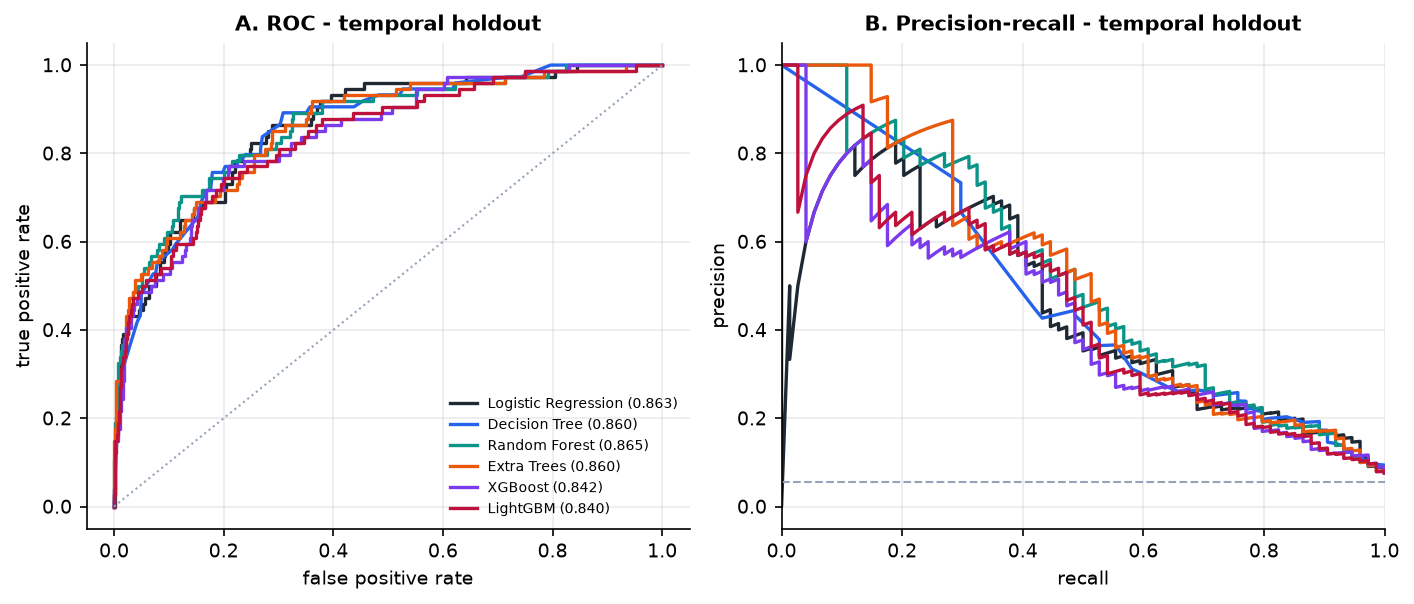
\includegraphics[width=\textwidth]{fig03_roc_pr_curves.png}
\caption{ROC curves (panel A) and precision-recall curves (panel B) on the temporal holdout. At this
prevalence the ROC panels compress into a narrow band while the precision-recall panels separate the
families.}
\label{fig:curves}
\end{figure}

\section{Calibration}

Predictions are well calibrated, with an expected calibration error of 0.016 and a Brier score of
0.0535: a stated risk of twenty-four per cent corresponds to an observed frequency near twenty-four
per cent. That is what makes a threshold-based alert defensible, since a message quoting a probability
must be numerically trustworthy.

\section{Ablation}
\label{sec:ablation}

Feature groups were removed and each configuration retrained (Table~\ref{tab:ablation}).

\begin{table}[htbp]
\centering
\caption{Ablation settings, using XGBoost with fixed hyperparameters.}
\label{tab:ablation}
\small
\begin{tabular}{@{}lccc@{}}
\toprule
\textbf{Feature set} & \textbf{Columns} & \textbf{PR-AUC (time)} & \textbf{PR-AUC (country)} \\
\midrule
History only & 7 & 0.407 & 0.174 \\
Population only & 14 & 0.432 & 0.241 \\
Climate only & 10 & 0.395 & 0.078 \\
Socio-geography only & 11 & 0.469 & 0.160 \\
History and population & 21 & 0.451 & 0.321 \\
All groups & 42 & 0.487 & 0.259 \\
All groups plus surveillance proxy & 44 & 0.497 & 0.261 \\
\bottomrule
\end{tabular}
\end{table}

Two results matter more than the headline. The reduced set of 21 columns reaches 0.321 under
leave-country-out validation, against 0.259 for the full 42: added covariates improve
in-distribution fit and reduce transfer by letting the model fit country peculiarities. Climate alone
reaches 0.078, marginally above the 5.59\% floor, so annual country climatology largely
encodes latitude and therefore country identity. Adding research-output proxies moves the
leave-country-out score by +0.001, weak evidence against pure publication tracking but not
proof.

\section{Chained Pipeline}

Table~\ref{tab:chain} reports the effect of appending the stage-one population forecast.

\begin{table}[htbp]
\centering
\caption{Effect of chaining the population forecast into the occurrence model.}
\label{tab:chain}
\small
\begin{tabular}{@{}lccc@{}}
\toprule
\textbf{Variant} & \textbf{PR-AUC (time)} & \textbf{ROC-AUC (time)} & \textbf{PR-AUC (country)} \\
\midrule
Plain (no chained feature) & 0.530 & 0.854 & 0.363 \\
Chained (population forecast added) & 0.527 & 0.853 & 0.344 \\
\bottomrule
\end{tabular}
\end{table}

The population forecast performs well as a forecast, with a mean absolute error of 0.424 on the log
scale and a Spearman correlation of 0.976. The intensity stage is weaker but usable, at a mean
absolute error of 0.150 and a rank correlation of 0.465 among positive observations. The hurdle
product ranks expected annual burden with a Spearman correlation of 0.326, and its highest decile
captures 70 of 106 observed events.

Appending the forecast changes temporal PR-AUC by -0.003, inside the noise band. The cause is
structural: population magnitude is already a direct feature, so forecasting it supplies a less
accurate copy of what the model holds. Chaining should help where that quantity cannot be observed
directly, which is not the case here.

\section{Alert Economics}

As a warning system, alerting the six per cent of country-years at highest predicted risk captures
about half of all observed events, and twenty-eight per cent captures eighty per cent
(Figure~\ref{fig:alerts}). Uniform alerting would need full coverage for the same recall, so the model
is roughly eight times more efficient than arbitrary selection at the fifty per cent point.

\begin{figure}[htbp]
\centering
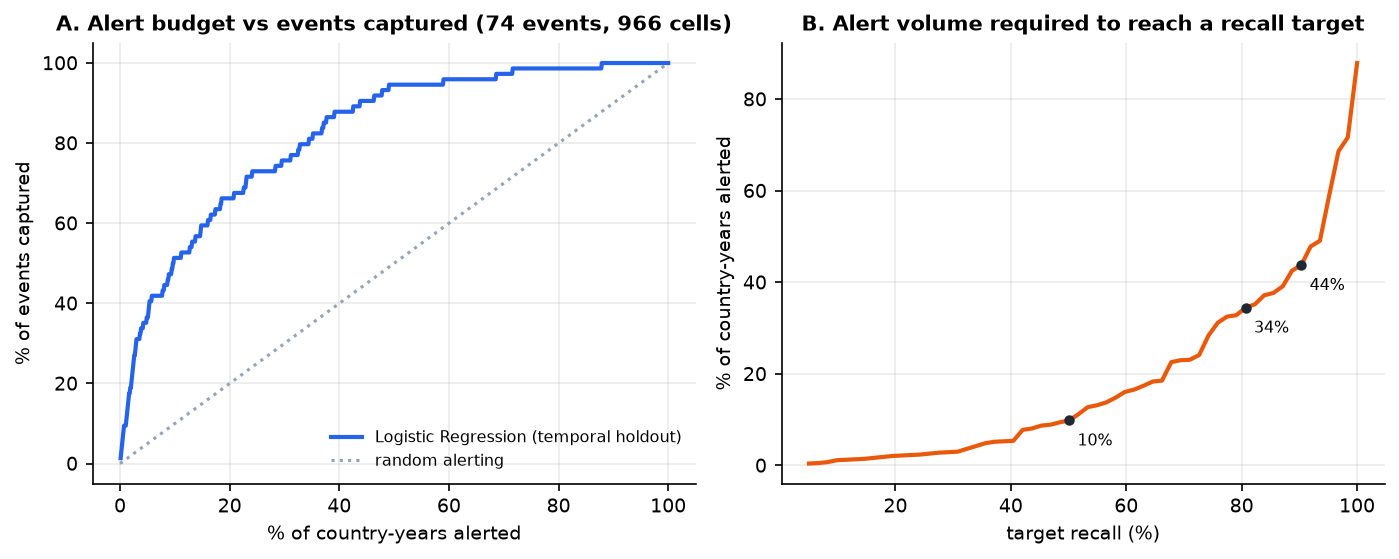
\includegraphics[width=0.78\textwidth]{fig07_alert_budget.png}
\caption{Alert economics. Panel A gives the fraction of events captured as the alert budget grows,
against random alerting. Panel B gives the alert volume required to reach a target recall.}
\label{fig:alerts}
\end{figure}

\section{Subgroup Analysis}

Table~\ref{tab:subgroup} reports leave-country-out performance by region. Skill is lowest in
Sub-Saharan Africa and in low-income countries, where early warning would help most. The cause is
label sparsity rather than a model defect: few events are recorded in those strata to learn from.

\begin{table}[htbp]
\centering
\caption{Leave-country-out performance by World Bank region.}
\label{tab:subgroup}
\small
\begin{tabular}{@{}lcccc@{}}
\toprule
\textbf{Region} & \textbf{Observations} & \textbf{Events} & \textbf{ROC-AUC} & \textbf{PR-AUC} \\
\midrule
East Asia \& Pacific & 456 & 48 & 0.865 & 0.396 \\
Europe \& Central Asia & 912 & 31 & 0.826 & 0.163 \\
Latin America \& Caribbean & 551 & 12 & 0.903 & 0.381 \\
MENA, Afghanistan and Pakistan & 380 & 23 & 0.834 & 0.220 \\
Sub-Saharan Africa & 665 & 27 & 0.699 & 0.073 \\
\bottomrule
\end{tabular}
\end{table}

\section{Discussion}

The model has predictive skill: a precision-recall AUC of 0.554 against a base rate of
5.59\% is not explainable by chance, survives a forward-looking split, and is calibrated to
within two points. It does not transfer intact, though: leave-country-out performance is roughly forty
per cent lower, and that is the planning figure, so a new country needs local validation first.

The principal signal is surveillance rather than biology, and three analyses agree: the highest
features are population and connectivity measures, the label concentrates in countries with reference
laboratories, and the best-scoring cells are India, the United States and Australia. Climate,
treated as a primary input in the proposal, transfers poorly here. Simpler models transfer better too,
which argues for parsimony when positives are few.

% =====================================================================
\chapter{Conclusion and Future Work}
\label{ch:concl}
% =====================================================================

\section{Conclusion}

This project set out to build a usable warning system for glanders: to establish whether
population-level risk could be predicted from public data, and to design how a prediction reaches the
person who owns the animals. Four sources not previously applied to the disease formed a country-year
panel across 162 equine-holding countries, six model families were trained under three validation
schemes, and a three-stage chained pipeline was tested. Around the model, delivery was decomposed into
three components with fixed contracts: a risk engine, a retrieval-augmented explanation layer and an
alert service.

Prediction is possible, and the performance is moderate. On a forward-looking temporal holdout the
strongest model reaches a precision-recall AUC of 0.554 against a base rate of 5.59\%, an
approximately 10-fold lift, with a calibration error of 0.016, capturing half of all observed
events while alerting six per cent of country-years. The skill is fragile across geography, though:
leave-country-out performance is about forty per cent lower, and the decline concentrates where early
warning would help most.

What the model learns is less encouraging. Three analyses converge: the highest-ranked features are
population size and reporting capacity rather than biological drivers, the label concentrates in
countries operating reference laboratories, and the best-scoring cells have the strongest publishing
record. It predicts where glanders will be documented, not where the organism is present. The chained
design does not improve discrimination because the intermediate quantity is already a direct feature.

The decomposition also proved useful: three components with versioned contracts, none hardcoding the
disease, were each testable alone, so the risk engine could be evaluated before any explanation
existed and the alert rules checked against a policy before any message was sent.

\section{Future Work}

\textbf{Reported activity.} The most important extension is to model surveillance capacity as a
quantity, as an offset on publication volume or through a two-part model estimating detection and
occurrence jointly; otherwise gains in score reflect reporting rather than disease.

\textbf{The label extractor.} The 263 extracted events have not been checked against a hand-annotated
set; annotating a stratified sample would give the extractor's own precision and recall, bounding
label noise that propagates downstream.

\textbf{Resolution.} The proposal envisaged district-month resolution for India; public district
covariates would need assembling, but that resolution matches the scale at which control is applied.

\textbf{The unmeasured components.} The calibration here is one point estimate; production needs
drift monitoring and a retraining trigger. The RAG layer's retrieval, guardrail and protocol targets
are specified but unmeasured, and running it against the corpus would give recall@5, faithfulness,
citation precision and the false refusal rate. \textbf{The field.} Messages per subscriber per year
decides whether the service survives a second year; a district pilot would supply it. A WOAH WAHIS
record set \cite{wahis} would validate the literature-derived label where the two overlap, and a
cost-sensitive threshold would match the operating point to the programme's priorities.

% ============================== REFERENCES ==============================
\newpage
\chapter*{Bibliography}
\addcontentsline{toc}{chapter}{Bibliography}
\renewcommand{\bibname}{}
\begin{multicols}{2}
\begin{thebibliography}{99}
\footnotesize
\setlength{\itemsep}{0.15em}
\setlength{\parskip}{0pt}
\bibitem{khan2013} Khan I, Wieler LH, Melzer F, et al. Glanders in animals: a review on epidemiology, clinical presentation, diagnosis and countermeasures. \emph{Transboundary and Emerging Diseases}. 2013. doi:10.1111/j.1865-1682.2012.01342.x
\bibitem{kanani2026} Kanani Y, Oryan A, Derakhshandeh A. Glanders: past, present and future of a neglected zoonosis as a threat in veterinary and human health. \emph{Veterinary Medicine and Science}. 2026. doi:10.1002/vms3.70950
\bibitem{purnama2026} Purnama MTE, Firdausy LW, Fikri F, et al. Seroprevalence and associated epidemiological drivers of glanders in horses: a systematic review and meta-analysis. \emph{Research in Veterinary Science}. 2026;106416. doi:10.1016/j.rvsc.2026.106416
\bibitem{mota2022} Mota RA, Pinheiro J\'unior JW. Current status of glanders in Brazil: recent advances and challenges. \emph{Brazilian Journal of Microbiology}. 2022. doi:10.1007/s42770-022-00814-1
\bibitem{singha2026} Singha H, Shanmugasundaram K, Jhandai P, et al. Surveillance of equine glanders in India (2019--2023): prevalence estimate, risk analysis and future strategy. \emph{Microbial Pathogenesis}. 2026;217:108597. doi:10.1016/j.micpath.2026.108597
\bibitem{singha2020} Singha H, Shanmugasundaram K, Tripathi BN, et al. Serological surveillance and clinical investigation of glanders among indigenous equines in India from 2015 to 2018. \emph{Transboundary and Emerging Diseases}. 2020. doi:10.1111/tbed.13475
\bibitem{malik2012} Malik P, Singha H, Khurana SK, et al. Emergence and re-emergence of glanders in India: a description of outbreaks from 2006 to 2011. \emph{Veterinaria Italiana}. 2012. PMID:22718333
\bibitem{fonseca2019} Fonseca-Rodr\'iguez O, Pinheiro J\'unior JW, Mota RA. Spatiotemporal analysis of glanders in Brazil. \emph{Journal of Equine Veterinary Science}. 2019. doi:10.1016/j.jevs.2019.03.216
\bibitem{hollings2017} Hollings T, Robinson A, van Andel M, et al. Species distribution models: a comparison of statistical approaches for livestock and disease epidemics. \emph{PLOS ONE}. 2017;12(8):e0183626. doi:10.1371/journal.pone.0183626
\bibitem{alshatti2026} Alshatti M, Al-Hemoud A, Othman A, et al. A risk prediction model for highly pathogenic avian influenza outbreaks in Kuwait. \emph{Frontiers in Veterinary Science}. 2026. doi:10.3389/fvets.2026.1843962
\bibitem{kane2014} Kane MJ, Price N, Scotch M, Rabinowitz P. Comparison of ARIMA and Random Forest time series models for prediction of avian influenza H5N1 outbreaks. \emph{BMC Bioinformatics}. 2014;15:276. doi:10.1186/1471-2105-15-276
\bibitem{walsh2019} Walsh DP, Ma TF, Ip HS, Zhu J. Artificial intelligence and avian influenza: using machine learning to enhance active surveillance for avian influenza viruses. \emph{Transboundary and Emerging Diseases}. 2019. doi:10.1111/tbed.13318
\bibitem{yoo2022} Yoo DS, Song YH, Choi DW, et al. Machine learning-driven dynamic risk prediction for highly pathogenic avian influenza at poultry farms in the Republic of Korea. \emph{Transboundary and Emerging Diseases}. 2021. doi:10.1111/tbed.14419
\bibitem{moawad2019} Moawad AA, Silge A, Bocklitz T, Fischer K, R\"osch P, Roesler U, Elschner MC, Popp J, Neubauer H. A machine learning-based Raman spectroscopic assay for the identification of \emph{Burkholderia mallei} and related species. \emph{Molecules}. 2019;24(24):4516. doi:10.3390/molecules24244516
\bibitem{stoeckel2015} St\"ockel S, Meisel S, Elschner M, Melzer F, R\"osch P, Popp J. Raman spectroscopic detection and identification of \emph{Burkholderia mallei} and \emph{Burkholderia pseudomallei}. \emph{Analytical and Bioanalytical Chemistry}. 2015;407(3):833--843. doi:10.1007/s00216-014-7906-5
\bibitem{collier2012} Collier N. Uncovering text mining: a survey of current work on web-based epidemic intelligence. \emph{Global Public Health}. 2012. doi:10.1080/17441692.2012.699975
\bibitem{lejeune2015} Lejeune G, Brixtel R, Doucet A, et al. Multilingual event extraction for epidemic detection. \emph{Artificial Intelligence in Medicine}. 2015. doi:10.1016/j.artmed.2015.06.005
\bibitem{chen2016} Chen T, Guestrin C. XGBoost: a scalable tree boosting system. In: \emph{Proceedings of the 22nd ACM SIGKDD International Conference on Knowledge Discovery and Data Mining}. 2016:785--794. doi:10.1145/2939672.2939785
\bibitem{ke2017} Ke G, Meng Q, Finley T, et al. LightGBM: a highly efficient gradient boosting decision tree. In: \emph{Advances in Neural Information Processing Systems 30 (NIPS)}. 2017:3146--3154.
\bibitem{breiman2001} Breiman L. Random forests. \emph{Machine Learning}. 2001. doi:10.1023/A:1010933404324
\bibitem{lundberg2017} Lundberg SM, Lee SI. A unified approach to interpreting model predictions. In: \emph{Advances in Neural Information Processing Systems 30 (NIPS)}. 2017:4765--4774. arXiv:1705.07874
\bibitem{saito2015} Saito T, Rehmsmeier M. The precision-recall plot is more informative than the ROC plot when evaluating binary classifiers on imbalanced datasets. \emph{PLOS ONE}. 2015;10(3):e0118432. doi:10.1371/journal.pone.0118432
\bibitem{davis2006} Davis J, Goadrich M. The relationship between precision-recall and ROC curves. In: \emph{Proceedings of the 23rd International Conference on Machine Learning}. 2006:233--240. doi:10.1145/1143844.1143874
\bibitem{roberts2017} Roberts DR, Bahn V, Ciuti S, et al. Cross-validation strategies for data with temporal, spatial, hierarchical, or phylogenetic structure. \emph{Ecography}. 2017. doi:10.1111/ecog.02881
\bibitem{niculescu2005} Niculescu-Mizil A, Caruana R. Predicting good probabilities with supervised learning. In: \emph{Proceedings of the 22nd International Conference on Machine Learning}. 2005:625--632. doi:10.1145/1102351.1102430
\bibitem{huang2020} Huang Y, Li W, Macheret F, et al. A tutorial on calibration measurements and calibration models for clinical prediction models. \emph{Journal of the American Medical Informatics Association}. 2020;27(4):621--633. doi:10.1093/jamia/ocz228
\bibitem{lewis2020} Lewis P, Perez E, Piktus A, et al. Retrieval-augmented generation for knowledge-intensive NLP tasks. In: \emph{Advances in Neural Information Processing Systems 33 (NeurIPS)}. 2020:9459--9474. arXiv:2005.11401
\bibitem{reimers2019} Reimers N, Gurevych I. Sentence-BERT: sentence embeddings using Siamese BERT-networks. In: \emph{Proceedings of the 2019 Conference on Empirical Methods in Natural Language Processing (EMNLP-IJCNLP)}. 2019:3982--3992. doi:10.18653/v1/D19-1410
\bibitem{malkov2020} Malkov YA, Yashunin DA. Efficient and robust approximate nearest neighbor search using hierarchical navigable small world graphs. \emph{IEEE Transactions on Pattern Analysis and Machine Intelligence}. 2020;42(4):824--836. doi:10.1109/TPAMI.2018.2889473
\bibitem{robertson2009} Robertson S, Zaragoza H. The probabilistic relevance framework: BM25 and beyond. \emph{Foundations and Trends in Information Retrieval}. 2009;3(4):333--389. doi:10.1561/1500000019
\bibitem{cormack2009} Cormack GV, Clarke CLA, Buettcher S. Reciprocal rank fusion outperforms Condorcet and individual rank learning methods. In: \emph{Proceedings of the 32nd International ACM SIGIR Conference}. 2009:758--759. doi:10.1145/1571941.1572114
\bibitem{pedregosa2011} Pedregosa F, Varoquaux G, Gramfort A, et al. Scikit-learn: machine learning in Python. \emph{Journal of Machine Learning Research}. 2011;12:2825--2830.
\bibitem{wahis} WOAH. World Animal Health Information System (WAHIS). \url{https://wahis.woah.org}
\bibitem{dahd2025} Department of Animal Husbandry and Dairying, Government of India. \emph{National Action Plan for Control and Eradication of Glanders in India} (Revised 2025). New Delhi: DAHD; 2025.
\bibitem{faostat} FAO. FAOSTAT: crops and livestock products. \url{https://www.fao.org/faostat}
\bibitem{power} NASA Langley Research Center. POWER agroclimatology API. \url{https://power.larc.nasa.gov}
\bibitem{wdi} World Bank. World Development Indicators. \url{https://databank.worldbank.org}
\bibitem{europepmc} Europe PMC literature search API. \url{https://europepmc.org}
\bibitem{nadres} ICAR-National Institute of Veterinary Epidemiology and Disease Informatics. National Animal Disease Referral Expert System (NADRES v2): livestock disease forecasting. \url{https://nivedi.res.in/Nadres_v2/}
\end{thebibliography}
\end{multicols}


\end{document}
